% !TEX root = presentation.tex
\section{Background}
\subsection{Machine Learning}
\frame{\frametitle{Machine Learning}
  \begin{itemize}
    \item Machine learning is a branch of \alert{artificial intelligence}.
    \item Focuses on the ability to \alert{classify} complex data.
    \item Uncover \alert{patterns} that characterize the data.
    \item Can \alert{train} on known data to \alert{predict} on unknown data.
  \end{itemize}
}

\subsubsection{Evaluating Applications of Machine Learning}
\frame{\frametitle{Evaluating Applications of Machine Learning}
  \begin{itemize}
    \item How do you \alert{measure} the \alert{performance} of your clustering/classification algorithm~\footnote{Requires data to have known categories}.?
    \begin{itemize}
      \item \alert{Compare} determined category vs. known category.
      \item Use a \alert{confusion matrix} and known measures.
      \item Use \alert{cross-validation}
    \end{itemize}
  \end{itemize}
}

\subsubsection{Confusion Matrix}
\frame{\frametitle{Confusion Matrix}
  \begin{figure}[!tb]
    \centering
    \begin{tikzpicture}[
    box/.style={draw,rectangle,minimum size=1.75cm,text width=4.0cm,align=center}]
      \matrix (confusion_matrix) {
        \node (actual_positive_prediction_positive)
        [box,
          label=left:\texttt{A},
          label=above:\texttt{A}
        ] {\underline{True Positives (TP)} \\ \textit{\scriptsize{\texttt{A} correctly classified as \texttt{A}}}};
        \pgfmatrixnextcell
        \node (actual_positive_prediction_negative)
        [box,
          label=above:\texttt{B}
        ] {\underline{False Negatives (FN)} \\ \textit{\scriptsize{\texttt{A} incorrectly classified as \texttt{B}}}};
        \\
        \node (actual_negative_prediction_positive)
        [box,
          label=left:\texttt{B}
        ] {\underline{False Positives (FP)} \\ \textit{\scriptsize{\texttt{B} incorrectly classified as \texttt{A}}}};
        \pgfmatrixnextcell
        \node (actual_negative_prediction_negative)
        [box] {\underline{True Negatives (TN)} \\ \textit{\scriptsize{remaining categories correctly classified not as \texttt{A}}}};
        \\
      };
      \node [left=-.1cm of confusion_matrix,text width=1.5cm,align=right] {\textbf{Actual \\ Value}};
      \node [above=-.1cm of confusion_matrix] {\textbf{Prediction Value}};
    \end{tikzpicture}
    \caption{A $2~\times~2$ confusion matrix for classification results of the \texttt{A} category.}
    \vspace{1mm}
    \footnotesize{\textit{It is possible to extend a confusion matrix to $n~\times~n$ dimensions. For each category the (TP, FN, FP, and TN) variables need to be calculated.}}
    \label{fig:example_confusion_matrix}
  \end{figure}
}

\subsubsection{Machine Learning Performance Measures}
\frame{\frametitle{Machine Learning Performance Measures}
  \begin{itemize}
    \item \textbf{Accuracy} represents the fraction of all true predictions made that were correctly identified.
    \begin{equation}
      \textit{$\text{accuracy} = \frac{TP + TN}{TP + FP + FN + TN}$}
      \label{equ:accuracy}
    \end{equation}
    \item Other traditional performance measures:
    \begin{itemize}
      \item Precision.
      \item Recall.
      \item Specificity.
     \end{itemize}
    \item More sophisticated performance measures:
    \begin{itemize}
      \item F-score.
      \item Balanced Accuracy.
      \item Youden's Index.
     \end{itemize}
  \end{itemize}
}

\subsubsection{Cross-Validation}
\frame{\frametitle{Cross-Validation}
  \begin{itemize}
    \item Evaluation using \textit{n}-fold cross-validation:
    \begin{enumerate}
      \item \alert{Split data} into \textit{n} equal sections.
      \item Use \textit{n-1} sections for \alert{training set}.
      \item Use remaining section for \alert{test set}.
      \item \alert{Predict} on test set and determine performance.
      \item Repeat step 2--4 a total of \textit{n} times using \alert{different test sets}.
      \item Determine \alert{average value} of measured performances over the \textit{n} folds.
    \end{enumerate}
  \end{itemize}
}

\subsection{Support Vector Machine}
\frame{\frametitle{Support Vector Machine}
  \begin{itemize}
    \item A \alert{supervised} machine learning \alert{classification} technique.
    \item Models a \alert{feature space} constructed using a set of \alert{vectors}.
    \item Vectors have a set of \alert{attributes} and a \alert{category}.
  \end{itemize}
  \begin{figure}
    \centering
    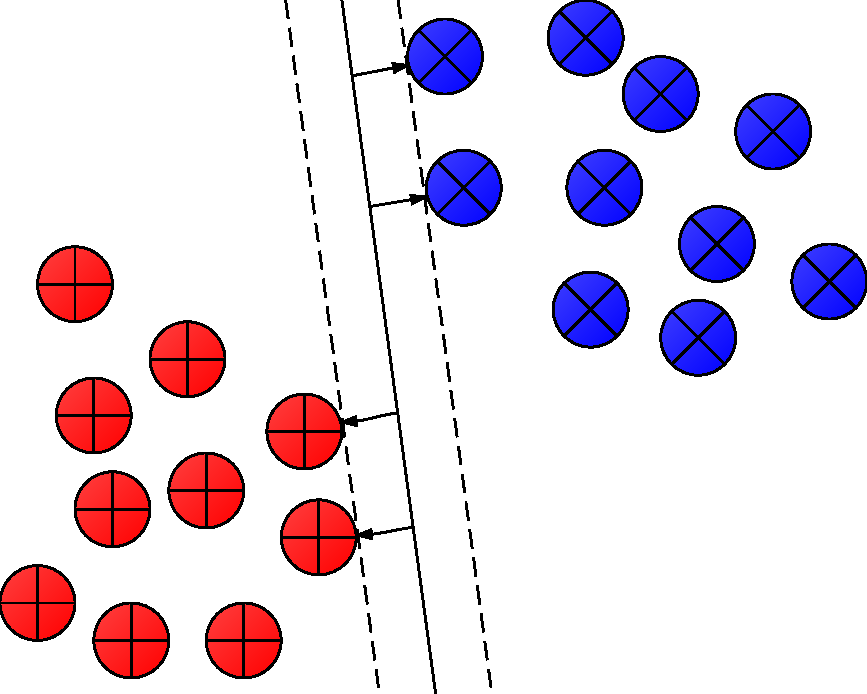
\includegraphics[width=4cm]{../thesis/figures/SVM_small_margin.pdf}
    $\xrightarrow{\texttt{Better Margin}}$
    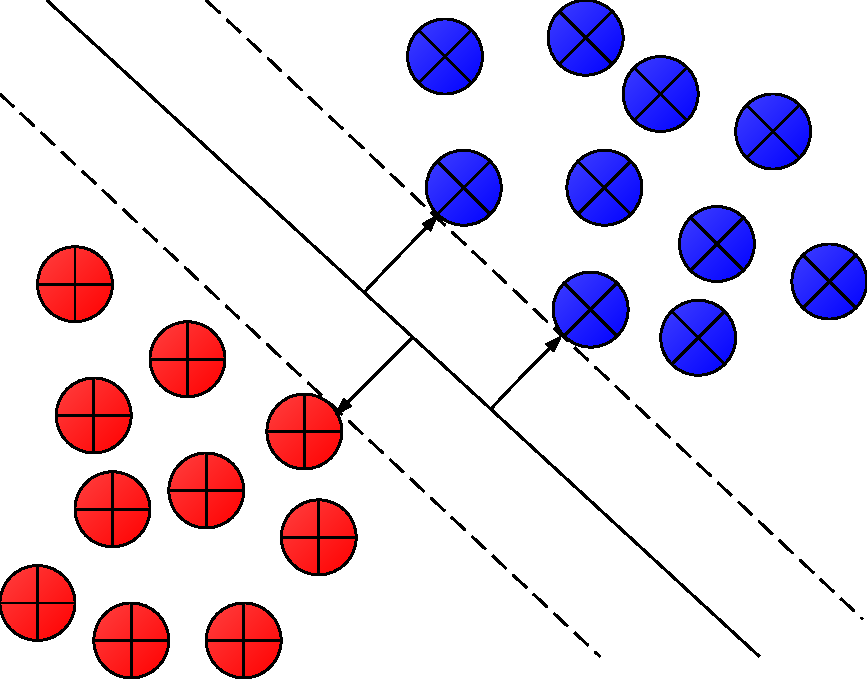
\includegraphics[width=4cm]{../thesis/figures/SVM_maximum_margin.pdf}
    \caption{A support vector machine attempts to \alert{linearly separate} vectors using a \alert{hyperplane}, such that the \alert{margin} is maximized.}
  \end{figure}
}

\subsubsection{Support Vector Machine Kernel Function}
\frame{\frametitle{Support Vector Machine Kernel Function}
  \begin{itemize}
    \item Works on \alert{non-linearly separable} data using \alert{kernel functions}.
  \end{itemize}
  \begin{figure}
    \centering
    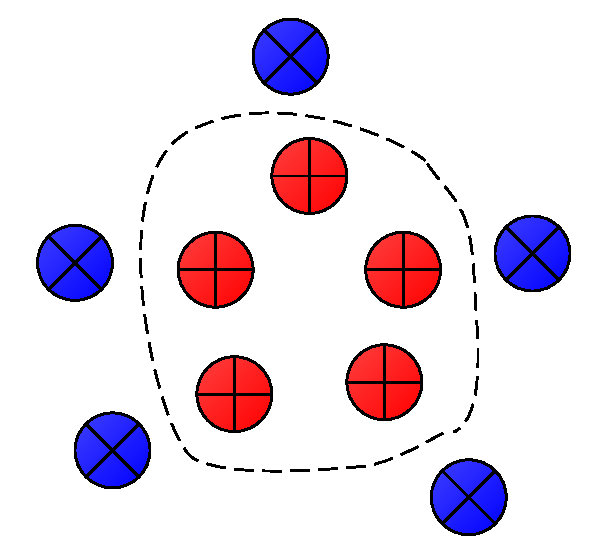
\includegraphics[width=3.5cm]{../thesis/figures/SVM_non-linear.pdf}
    $\xrightarrow{\texttt{Kernel Function}}$
    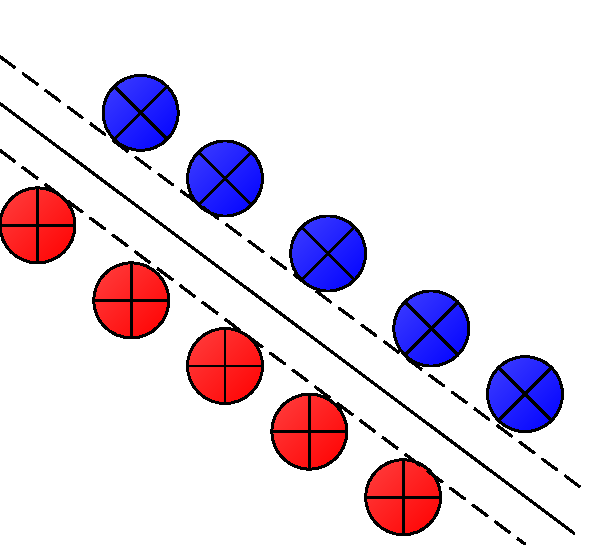
\includegraphics[width=3.5cm]{../thesis/figures/SVM_kernel_function.pdf}
    \caption{\alert{Map} feature space into a \alert{higher dimension} and attempt to linearly separate vectors.}
  \end{figure}
  \begin{itemize}
    \item Works for \alert{\textit{many}-group} classification.
  \end{itemize}
}

\subsection{Software Metrics}
\frame{\frametitle{Software Metrics}
  \begin{itemize}
    \item A \alert{software metrics} can be broken down into the following~\footcite{Fen94}:
    \begin{itemize}
      \item \textbf{Entity:} Represents an \alert{object} or \alert{event}.
      \item \textbf{Attribute:} Represents a \alert{feature} or \alert{property} of an \textit{entity}.
      \item \textbf{Model:} Represents a \alert{specific viewpoint} of an \textit{attribute}.
    \end{itemize}
    \item Example:
    \begin{itemize}
    	\item Entity: people
			\item Attribute: hieght
			\item Model: barefoot, back against wall, legs straight, hair down
		\end{itemize}
  \end{itemize}
}

\subsubsection{Source Code Metrics}
\frame{\frametitle{Source Code Metrics}
  \begin{itemize}
    \item Measure \alert{structural} aspects of the \alert{source code}.
    \item Typically done using \alert{static analysis} on the source code files.
    \begin{itemize}
      \item Complexity.
      \item Number of source lines of code.
      \item Maximum nested block depth in a method.
      \item Number of methods/classes.
      \item etc\ldots
    \end{itemize}
  \end{itemize}
}

\subsubsection{Test Suite Metrics}
\frame{\frametitle{Test Suite Metrics Metrics}
  \begin{itemize}
    \item Measure \alert{similar} structural aspects to \alert{source code metrics} (e.g., complexity, etc\ldots).
    \item Measure \alert{relationship} between \alert{test suite} and the \alert{software system under test}.
    \begin{itemize}
      \item Number of test cases for system/class/method.
      \item Statement/branch/decision coverage.
      \item etc\ldots
    \end{itemize}
  \end{itemize}
}
